\chapter{Deep Learning in Digital Histopathology}

We begin by introducing the field of histopathology and its concerns, alongside with tools and methods used in contemporary clinical practice. We show how digitization helped to reduce the logistical complexity of histopathologists workflow, and how decision support systems can further reduce the required human labor. We follow by introducing feed-forward artificial neural networks, with focus on convolutional networks, which are exceptional at tackling various computer vision problems.

\section{Histopathology}

Histopathology is a discipline concerned with study of diseases of tissue. This involves, but is not limited to cancer detection and prediction [], infectious or inflammatory disease diagnostics [] and study of brain-degenerative diseases such as Parkinson's or Alzheimer's [].

Histopathologists are medically qualified physicians, who inspect tissue taken from patients. Their expertise is essential in identifying cellular irregularities and tissue distortions that could indicate a range of medical conditions. Histopathologists often cooperate with other doctors, providing insights to help set the direction of further patients care [].

\section{Temporal and spatial limitations of traditional Histopathology}

Traditionally, to get tissue from patient to histopathologist, tedious logistic process involving several people is necessary. Surgeon needs to extract tissue samples from patient. Extracted tissue is then sent to specialized laboratory for processing -- in the laboratory, tissue samples are infused with mix of chemicals and embedded into paraffin wax block. The parafin block is then thinly sliced into sections of approx. $3$ microns, and those section are laminated onto a glass slide. Glass slides are further stained with hematoxilin/eosin (or other compound) [] to enhance contrast between different cellular structures. After the lab processing, slides are delivered to histopathologist for a review.

While we currently cannot replace surgeon performing the biopsy or lab workers staining and embedding the tissue, we can address logistic challenges of moving glass slides to histopathologist. Having a physical slide suffers from several inefficiencies. A slide can be studied only by one histopathologist at a time and if a second opinion from a different histopathologist is required, the glass slide must be conveyed to the respective clinic. This throttles the diagnosis process and leads to longer waiting times for a patient.

\section{Digital histopathology}

Digital histopathology aims to reduce the logistic overhead caused by physical copies of glass slides. After the tissue is extracted and prepared, instead of shipping it to a histopathologist, it is scanned using specialized lenses resulting in a high-resolution digital image, called \emph{Whole Slide Image} (WSI) [].

This image is then uploaded to an aggregator server, which enables real-time sharing of slides and parallel cooperation of multiple clinicians. Histopathologists then inspect WSI in a dedicated browsers on their computer monitors, instead of looking at the glass slide under a microscope. How a WSI can look in a browser is depicted in Figure \ref{fig:xopat}.

Even though contemporary digital pathology systems provide a significant speed up in pathologists day to day work, we can further optimize another productivity metric – pathologists time spent on inspection of WSIs. Recently, researches and various companies made attempts to employ machine learning systems to further aid pathologist during the diagnosis process. 

\begin{figure}[!h]
    \begin{center}
    \begin{minipage}{0.75\textwidth}
      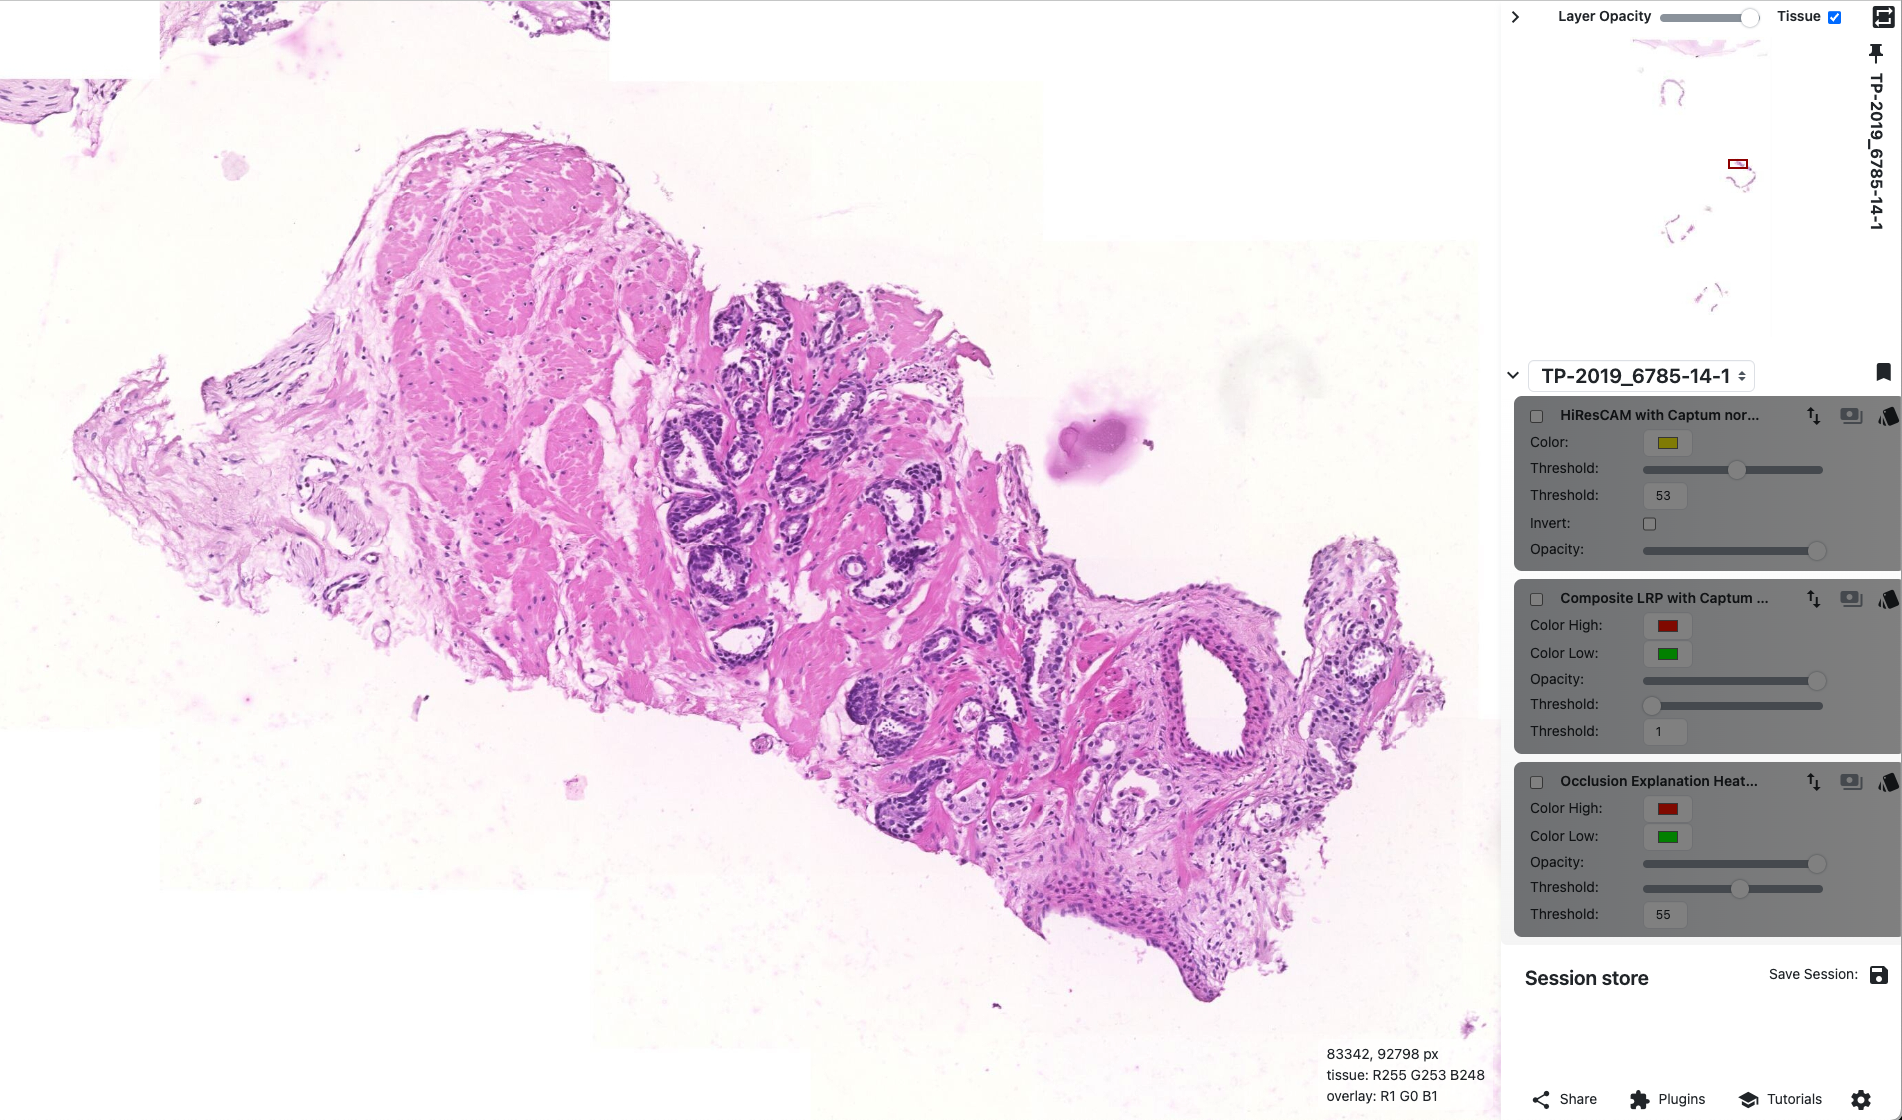
\includegraphics[width=\textwidth]{img/xopat.png}
    \end{minipage}
    \caption{xOpat [] WSI browser with a sample of prostate tissue. Histopathologist is able to move and zoom the tissue, allowing him to quickly navigate in the WSI. Having digitized copies allows for layering of arbitrary annotations on top of the WSI, providing great collaborative capabilities.}
    \label{fig:xopat}
    \end{center}
\end{figure}
\todo{Maybe add border?}

\subsection*{Decision Support System}

A computer system, which aids human to make a decision while performing a particular task is referred to as decision support system []. These systems are utilized across a wide array of applications, including high-stake environments such as investment banking [], autonomous driving [] or military and defense []. In digital histopathology, such systems are usually utilized to help with operational processes []. With deep learning in the spotlight of today's research, new possibilities emerge.

New systems could be utilized to enhance tissue diagnostic process by assisted diagnosis, or used to discover previously unrecognized features in large sets of data, incomprehensible by a single expert [].
%% https://pathsocjournals.onlinelibrary.wiley.com/doi/10.1002/path.5388
Random forests [], support vector machines [] and various neural network architectures [] are all attempts of such utilization. Those systems often provide real-time results and human-like performance, demonstrating that further research in this area can bring significant improvement to the contemporary processes [].

%% decision trees - https://www.researchgate.net/publication/363350224_Random_forest_modelling_demonstrates_microglial_and_protein_misfolding_features_to_be_key_phenotypic_markers_in_C9orf72-ALS
%% svm - https://www.ncbi.nlm.nih.gov/pmc/articles/PMC1924513/pdf/1471-2121-8-S1-S8.pdf
%% neural networks - https://arxiv.org/pdf/2312.02225.pdf
%%                 - https://www.sciencedirect.com/science/article/pii/S2666827021000992

\section{Deep Learning}
%% Brief intro to what is deep learning, methods and techniques? Common use cases of deep learning in digital histopathology.

Area of machine learning encapsulating neural networks is referred to as deep learning (DL). Methods and algorithms employed by DL achieve remarkable results across various domains, including computer vision [imagenet?], games [alphago], weather forecast [] and natural language processing [gpt].

Introduced in 1943 by McCulloch and Pitts [] with goal of creating a computational unit resembling a neuron in human brain, neural networks have come a long way to the prominent place they occupy today.

%% forecast - https://www.nature.com/articles/s41586-023-06185-3

\subsection*{Feed-forward Neural Network}

Neural networks can be seen as a specific arrangement of computational units called neurons. Feedforward networks, or multi-layer perceptrons (MLPs) are considered the foundation of contemporary models. We can see a MLP as a function $f$ that maps real-valued input vector \textbf{x} to a single value $y$. A MLP is a sequence of layers, and we can consider each layer $l$, to resemble intermediate function $f^l$. If our MLP has $L$ layers, given an input vector \textbf{x}, we can write $f(\textbf{x})$ as a composition of those intermediate functions, denoted by $f^L(f^{L-1}(...f^1(\textbf{x})))$. $f^1$ is the first layer of MLP, called input layer. $f^L$ is called output layer and all in-between layers are reffered to as hidden []. Even though ... shows that one hidden layer is all you need, it is common for MLPs to consist of multiple layers. The motivation is that each layer can be seen, as if it captures certain abstractions or patterns from its input. Deeper layers can build more complicated patterns by utilizing abstractions captured by previous layers. % Figure \ref{fig:simple-mlp} depicts a simple multi-layered perceptron (MLP) with one hidden layer.

Layer consists of its neurons. Each neuron has associated its weights and bias. In a feedforward network, weights only connect neurons in two consecutive layers. If all neurons in a given layer have a incoming weight from all neurons in the previous layer, we say that $l$ is fully-connected. Given neuron $j$ from layer $l$ and neuron $i$ from previous layer $l - 1$, we denote $w_{ji}$ as the weight from $i$ to $j$ and $b_j$ as the bias of neuron $j$. Additionally, each neuron has its activation function\footnote{Heaviside step function was the first activation function to be used. This led to a number of problems [] and because of their importance, activation functions are vital part of research interest up to this day [].}, commonly denoted as $\phi$. Given a neuron $i$ with activation function $\phi_i$, which has incoming weights from $K$ neurons in the previous layer, formula for a function $g_i$ computed by neuron $i$ can be written as:

\begin{equation}
y_i = \phi_i(\sum_{k=1}^K w_{ik}y_k)
\end{equation}

Deep learning aims to make networks weights and biases useful. Since a network computes a function $f$, with specific training, we can make network learn to approximate any desired function $f^*$ within a certain tolerance []. To train a network, we leverage large amount of data to adjust networks parameters to minimize difference between its and desired outputs. The difference is captured using loss function $\mathcal{L}$, and the process of minimizing $\mathcal{L}$ is typically performed iteratively using backpropagation and traning algorithm such as stochastic gradient descent. More on neural networks training can be found in []. 

Despite deep dive to training is out of scope of this thesis, we need to familiarize ourselves with the notion of partial derivatives. Partial derivatives are commonly used to find a direction in which we move certain weight $w$ to minimize the $\mathcal{L}$, if all other parameters remain fixed. We denote the partial derivative of $\mathcal{L}$ with respect to $w$ as $\frac{\delta \mathcal{L}}{\delta w}$. 

%% goodfellow kniha

\begin{figure}[!h]
    \begin{center}
    \begin{minipage}{.75\textwidth}
      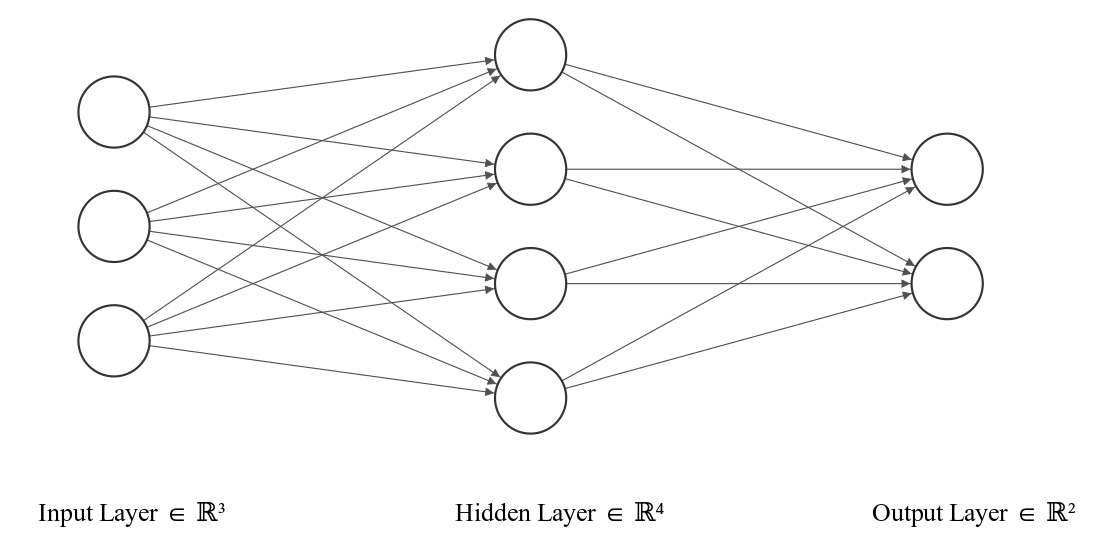
\includegraphics[width=\textwidth]{img/nn.png}
    \end{minipage}
    \caption{Architecture of a multi-layer perceptron with one hidden layer. Circles represent layer inputs. Edges represent layer weights. Biases are omitted for simplicity. Given a non-input layer L, if every unit has an incoming edge from all units in previous layer, we consider the perceptron to be fully-connected.}
    \label{fig:simple-mlp}
    \end{center}
\end{figure}

Even though MLPs demostrate impressive results on tasks previously deemed impossible for computers, they come with certain setbacks. Given fully connected layers, even small contemporary architectures such as ImageNET would have unimaginable number of trainable parameters. This led to development of new architectures, tailored to specific domain needs. Despite shift from using fully-connected layers only, MLP stood its ground and to this day, it is essential part of various state of the art neural network models [gpt, alexnet].

\subsection*{Convolutional Neural Network}
%% Architecture
Architecture introduced specifically to solve various computer vision problems adds two additional layer types --- convolutional and pooling. These layers help to capture patterns in input features, as well as reduce size of the network []. 
%% - https://arxiv.org/pdf/1511.08458.pdf

%% TODO: Why it suits them for image processing

\subsubsection{Convolutional Layer}

Convolutional layer searches for visual patterns in its input. It utilizes learnable filters (sometimes called kernels) typically significantly smaller in dimensions than the input. Instead of interacting with whole input at once using weights, as it is case for fully-connected layers, the filter with its own weights is instead systematically slid across the input. Weights of a filter are convolved with the corresponding input data segments, yielding an activation map. Resulting activation map can be seen as a evidence for presence of a shape, detected by the filter in the input data. Sliding filter through features gives us spatial invariance -- no matter where in the input the pattern is, it will get detected and reflected in a activation map, something very hard to achieve using fully-connected layer. Therefore it is commonly said, that the filter has "shared weights".

When incorporating a convolutional layer into a neural network, instead of specifying the number of neurons as with FC layers, the crucial parameter to define is the filter shape. This shape determines the receptive field's size -- how much of the input the filter can see at any given time. In addition we usually set two other parameters: \emph{padding} and \emph{stride}. Padding is a value we add as a border around the input features, allowing the filter to cover the edges and thus reducing information loss. Stride controls how much we shift the filter after each convolution. For visual representation of these concepts see Figure \ref{fig:cnn-convolution}.


\begin{figure}[!h]
    \begin{center}
    \begin{minipage}{0.75\textwidth}
      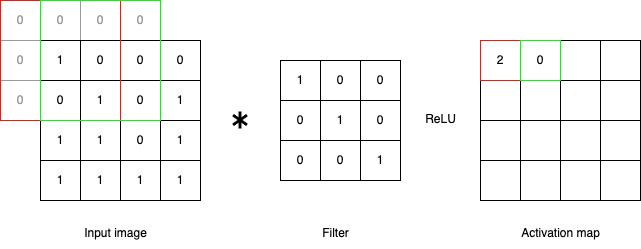
\includegraphics[width=\textwidth]{img/cnn-conv.png}
    \end{minipage}
    \caption{Example of simple calculation within convolution layer. Filter detects diagonal edge of lenght 3 pixels. Stride and padding are both set to 1 pixel and zero is used as the padded value. The result is passed through ReLU activation function.}
    \label{fig:cnn-convolution}
    \end{center}
\end{figure}

Convolutional layer consists of multiple units. Each unit has its own filter and produces unique activation map. The idea is that during training, each filter learns to recognize a different pattern. This gives a single layer capabilities to detect multiple patterns and similarly to its fully-connected counterpart -- it allows subsequent layers of the network to build upon captured abstractions and ultimately "understand" and represent high level concepts.

It is important to note, that sharing weights has not only effects of identifying patterns regardless of their position in the input -- it reduces the size of networks as well. Given $512$ input and output features, a fully connected layer needs $262,144$ weights to propagate the information. On the other hand, convolutional layer with $1,024$ units and receptive field of size $3 \times 3$ needs $9,216$.

\subsubsection{Pooling Layer}

To prevent overfitting, pooling layers are employed to further distill patterns captured by a CNN. They progressively reduce size of the features, leading to reduced number of model parameters and computational complexity [].

A pooling layer is typically placed after a convolutional one, iterating over its activation maps and applying systematically applying a specific operation over its receptive field. We differentiate between two primary types of pooling: \emph{max} and \emph{average}. As their names imply, max pooling selects the maximum value within its receptive field, while average pooling computes the mean of the values. Pooling layer has its own filters and strides, however, the parameters are chosen more conservatively. A common choice is $2 \times 2$ filter and stride of $2$, ensuring that the pooled sectors do not overlap. It has been observed, that having a filter of size greater than $3 \times 3$ will most likely lead to loss of model's performance, since such granularity may hide too of the features detected by a network [].

\begin{figure}[!h]
    \begin{center}
    \begin{minipage}{0.5\textwidth}
      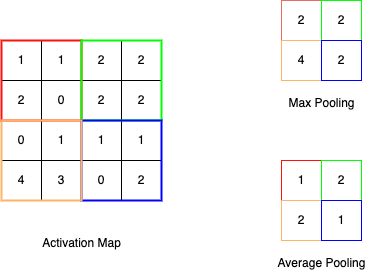
\includegraphics[width=\textwidth]{img/cnn-pool.png}
    \end{minipage}
    \caption{Example of both max and average pooling layers. Both have filters of size $2x2$ and stride set to $2$, resulting in no overlap during computation. Notice, that since each $2x2$ region is mapped to a single value, the new activation mask has quarter the features of the original.}
    \label{fig:cnn-pooling}
    \end{center}
\end{figure}

\subsubsection{Global Pooling Layer}

Given our network composed solely of convolutional and pooling layers, we are not bound to any specific input size -- thanks to the inherent spatial invariance. Nonetheless, it is common practice to introduce fully connected layers towards the end of the network, which require a fixed-size number of input features. To meet this requirement, we use global pooling layers.

Similar to standard pooling, global pooling comes in two forms: max and average. Global pooling layers operates on each activation map, condensing it into a single value. This guarantees that if a convolutional layer has $n$ units and the subsequent fully-connected layer receives $n$ input features, placing a global pooling layer in between will provide a compatible transition, standardizing the output size regardless of the input dimensions.
